%%%%%%%%%%%%%%%%%%%%%%%%%%%%%% -*- Mode: Latex -*- %%%%%%%%%%%%%%%%%%%%%%%%%%%%
%% 00slides.tex 
%% Author          : Yaakov Oshman
%% Created On      : Thu Apr 15 22:28:37 2004
%% Last Modified By: Yaakov Oshman
%% Last Modified On: Thu Feb 11 16:39:30 2010
%% Update Count    : 412
%% Status          : Unknown, Use with caution!
%%%%%%%%%%%%%%%%%%%%%%%%%%%%%%%%%%%%%%%%%%%%%%%%%%%%%%%%%%%%%%%%%%%%%%%%%%%%%%%
        
%% PROCESSING THE LATEX FILE (use both input and output file names!):
%%    1. latex file.tex
%%    2. dvips -ta4 -Ppdf file.dvi -o file.ps  (a4 page size)
%%    3. ps2pdf -r1200 file.ps file.pdf (1200 resolution)

       
\documentclass[mathserif]{beamer}
%%\documentclass[gray,handout,mathserif]{beamer}

%%\documentclass[mathserif,allowframebreaks,shrink]{beamer}
%% frame options:
%%  
%% [squeeze] for squeezing vertical space
%% [shrink] for shrinking the content to fit in a single slide
%% \frame[plain]{\frametitle{}...} for plane frame style
%% [allowframebreaks] automatic splitting of frame if content does not
%% fit in a single slide


%\usetheme{split}    % takes more vertical space!!
%\usetheme{Berkeley} % vertical side navigation bar
%\usetheme{Malmoe}
%\usetheme{shadow}
%\usetheme{PaloAlto}  %  side nav bar
%\usetheme{Copenhagen}  %  top nav bar
%\usetheme{Madrid}  %  no nav bar
\usetheme{Boadilla}  % nice and clean, no nav bar, max space!
%\usetheme{montpellier}  %  top tree
%\usetheme{Singapore}  %  top (sort of tree)
%\usetheme{pittsburgh}   % no nav bar, clean, takes more space than Boadilla...
%\usetheme{szeged}

\setbeamertemplate{navigation symbols}{}  %no nav symbols at bottom of PDF
%% or
%% \usenavigationsymbolstemplate{}
%%



\usepackage{eulervm}
%%\usepackage[small]{eulervm}

%%\beamertemplateballitem    %% fancy bulletts

\usepackage{colordvi}  %% texmf/tex/generic/dvips/colordvi.tex (names
                       %% of all predefined colors)

\usepackage{amsmath}
\usepackage{amssymb}
\usepackage{amsfonts}
\usepackage{amsthm}
\usepackage{bm}
\usepackage{xspace}
\usepackage{latexsym}
\usepackage{mathrsfs}
\usepackage{wasysym}
%\usepackage{arydshln}
\usepackage{eulervm}
\usepackage[T1]{fontenc}
\usepackage{aurical}


\graphicspath{{Figures/}}
\DeclareGraphicsRule{*}{eps}{*}{}
%\DeclareGraphicsExtensions{.eps}

\newcommand{\epspath}{}
%\newcommand{\epspath}{g:/usr1/etc/logos/}
   
\newenvironment{slidelist}{\begin{list}{$\bullet$}%
    {\itemsep -0.5ex \topsep -2ex \partopsep 0ex}}{\end{list}}

\newenvironment{smilebullet}{\begin{list}{{\large \green \smiley}}%
{\itemsep 1ex \partopsep 0ex}}{\end{list}}

\newenvironment{frownbullet}{\begin{list}{{\large \green \frownie}}%
{\itemsep 1ex  \partopsep 0ex}}{\end{list}}

\newcommand{\subheading}[1]{\textbf{\textsf{{\textcolor{blue}{#1}}}}}
\newcommand{\subsubheading}[1]{\textbf{\textsf{\textcolor{red}{#1}}}}

\newcommand{\BLOM}{{\bf BLOM }} 

\title[\BLOM]{{\bf BLOM}: {\bf B}erkeley {\bf L}ibrary for \\ 
  {\bf O}ptimization {\bf M}odeling}
%
\author[S. Vichik, A. Kelman]{Sergey Vichik
%
  ~and~Anthony Kelman }


\date[January 2013]{January, 2013}

\institute[UC Berkeley]{UC Berkeley\\
  Department of Mechanical Engineering\\
  Berkeley, CA \\[1ex]
  \{sergv, kelman\}@berkeley.edu \hspace{1em}}

%

\renewcommand{\include}{\input}       


         
\begin{document}

%
\begin{frame}
  \titlepage
\end{frame}
%

%\begin{frame} \frametitle{Outline}
%  \tableofcontents
%\end{frame}
%
%\include{abstract}
%%\tableofcontents[current]

\begin{frame}
\frametitle{What is \BLOM ?}
\begin{itemize}
\item A {\bf tool} and {\bf language} of modeling
(dynamical) nonlinear systems for optimization problems.
\item Conventional approach
\begin{itemize}
\item	Manual formulation and coding
\item  Time consuming, error prone (especially gradients, Jacobian, Hessian)
\item	Difficult to change solvers
\item	Tricky to get good performance
\end{itemize}
\item \BLOM approach eliminates manual problem coding, eases maintenance and assures that the
  same model used for optimization as for simulation
\begin{itemize}
\item Developing the model with an intuitive block diagram
\item Simulink/Matlab based interface.
\item Forward simulation for validation of the model
\item Developed to handle non trivial problems
\begin{itemize}
\item Explicit evaluation of Jacobian and Hessian
\item Automatic and efficient export of the optimization problem to a solver
\end{itemize}
\end{itemize}
\end{itemize}
\end{frame}

\begin{frame}
\frametitle{''Hello World'' model example}

\centering 
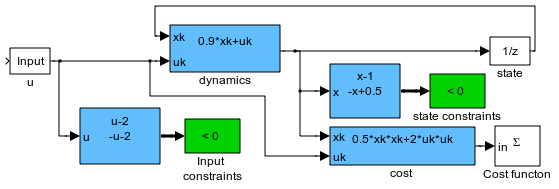
\includegraphics[width = .7\textwidth]{HelloWorld}
\begin {align}
\min_{u_k,x_k}& \sum_k 0.5x_k^2 + 2u_k^2 \notag \\
s.t.:&  -2 \leq u_k \leq 2 \ ; 0.5 \leq x_k \leq 1\ ; x_{k+1}=0.9x_k+u_k \notag
\end{align}

\begin{itemize}
\item The \alert{Functional} block holds expression of the form $\frac{f(x)}{g(x)}$   
\item The \alert{Constraint} block marks variable as $\geq 0$ or $\leq 0$
\item The continuous or discrete \alert{State} block
\item The \alert{Cost} block accumulates cost variables over horizon
\item The \alert{Input/External} variable modifiers marks the control and the
  external variables
\end{itemize}
\end{frame}

\begin{frame}
\frametitle{Eficient problem representation}

\begin{itemize}
\item	Why are LP, QP easy?
\begin{itemize}
\item	Standard format, 	e.g. for QP:
\begin{align*} 
\min_x  \ \frac{1}{2} & x^TQx + c^Tx \\ \text{s.t.} \ & A x \leq b \\ & Ex = d  
\end{align*}
\item	Gradient, Jacobian, etc immediate
\end{itemize}
\item Typical nonlinear approach:
\begin{itemize}
\item	Code generation or parsing, algorithmic differentiation
\item	Explicit code gen does not scale well to very large problems
\end{itemize}
\item	\BLOM is our proposal for standardized NLP format
\begin{itemize}
\item	Represent nonlinear structure of model in sparse matrices
\item	Matrix of exponents/functions, matrix of coefficients
\item	Cost vector, upper and lower bound vectors
\end{itemize}
\item 	\alert{Key to performance of optimization algorithms}
\end{itemize}
\end{frame}

\begin{frame}
\frametitle{ \BLOM representation details}
\begin{gather*}
f(x) = \sum_{k=1}^r K_{k} \left( \prod_{j=1}^n v(x_j, P_{kj}) \right) 
\label{eq:polyblock_eq}
\end{gather*}
The parameterized function $v$ is defined as
\begin{equation*}
v(x, p) = \left\{ \begin{array}{cl}
x^p & \text{if } p \text{ is not an exception code} \\
\exp(x) & \text{if } p \text{ is the code for } \exp \\
\sin(x) & \text{if } p \text{ is the code for } \sin \\
\tanh(x) & \text{if } p \text{ is the code for } \tanh \\
\text{etc.} \vspace{-10pt}
\end{array} \right.
\label{eq:v_definition}
\end{equation*}
\begin{itemize}
\item	Multivariate polynomial-like structure with sparse P, K
\item	Closed-form sparse Jacobian, Hessian
\end{itemize}
\end{frame}


\begin{frame}
\frametitle{\BLOM work flow}
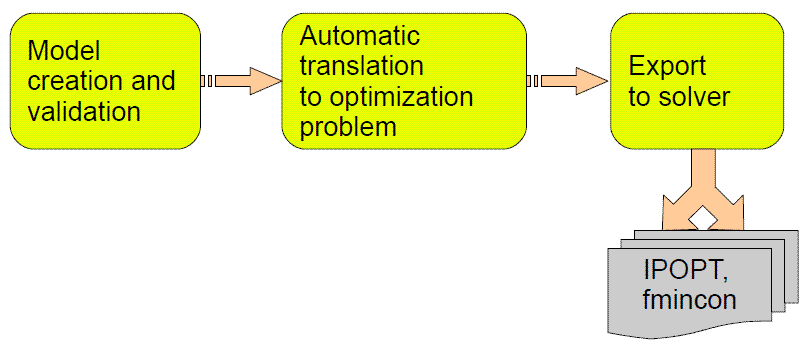
\includegraphics[width=0.9\textwidth]{WorkFlowBlom}

\begin{itemize}
\item Create model using Simulink with \BLOM library
\item Run and compare the model to reference data
\item Automatically generate efficient problem representation
\item Compiled interface to optimization solvers
\end{itemize}

\end{frame}

\begin{frame}
\frametitle{Availability, License and Usage}
\begin{itemize}
\item 	Publicly available since September
 \\
	Follow links at {\color{blue} www.mpc.berkeley.edu}, under Software BSD license: free to use, modify, or redistribute
\item 		Please cite us if you find it useful
	(as academic courtesy, not a condition of license)
\item 		Not application specific, feel free to evaluate for other projects
\item 		Being used in large HVAC MPC setup by UTRC, Master's level MPC course at Berkeley, HVAC MPC in our lab, wave energy conversion research
\item    Typical computation times from $0.3$~sec for $\sim 1000$~variables to $\sim 100$~sec for $\sim 30k$~variables 
\end{itemize}

\end{frame}

\begin{frame}
\frametitle{Ongoing development}
\begin{itemize}
\item	Top priority: allow models constructed from built-in Simulink blocks -- products, sums, nonlinear functions
\item	Would be able to take preexisting Simulink models (if simple), just mark cost, constraints, and inputs
\item	Improved documentation, including quick-start guide
\item	Code cleanup for better data structures, readability
\item	Interface to more optimization solvers, languages
\item	Thorough benchmarking vs other similar tools
\item	Simpler mechanism for terminal constraints and cost
\item	Norms over vector elements or time for cost, constraints
\item	Discretization enhancements, fixes, more methods
\end{itemize}
\end{frame}


\begin{frame}
\frametitle{Summary}
\begin{itemize}
\item	BLOM eliminates manual coding of optimization model, facilitates very fast development cycle
\item	High performance for very large scale models
\item	Simplifies collaborative development and knowledge transfer between team members -
\\
	Using someone else's block diagram vs reading their code
\item	Develop model once, use with any solver and environment later
\end{itemize}

\end{frame}


\end{document}

\endinput

